%%%%%%%%%%%%%%%%%%%%%%%%%%%%%%%%%%%%%%%%%%%%%%%%%%%%%%%%%%%%%%%
% Welcome to the MAT320 Homework template on Overleaf -- just edit your
% LaTeX on the left, and we'll compile it for you on the right.
%%%%%%%%%%%%%%%%%%%%%%%%%%%%%%%%%%%%%%%%%%%%%%%%%%%%%%%%%%%%%%%
% --------------------------------------------------------------
% Based on a homework template by Dana Ernst.
% --------------------------------------------------------------
% This is all preamble stuff that you don't have to worry about.
% Head down to where it says "Start here"
% --------------------------------------------------------------

\documentclass[12pt]{article}

\usepackage{graphicx}
\graphicspath{{./images/}}
\usepackage{textcomp} % cent symbol, such as \textcent
\usepackage[margin=1in]{geometry} 
\usepackage{amsmath,amsthm,amssymb}
\usepackage{mathtools} % ceiling function
\DeclarePairedDelimiter{\ceil}{\lceil}{\rceil}
% https://tex.stackexchange.com/questions/146306/how-to-make-horizontal-lists
\usepackage[inline]{enumitem} % allows using letters in enumerate list environment

% source: https://stackoverflow.com/questions/3175105/inserting-code-in-this-latex-document-with-indentation

\usepackage{listings}
\usepackage{color}

\definecolor{dkgreen}{rgb}{0,0.6,0}
\definecolor{gray}{rgb}{0.5,0.5,0.5}
\definecolor{mauve}{rgb}{0.58,0,0.82}

\lstset{frame=tb,
	language=VHDL, % language for code listing
	aboveskip=3mm,
	belowskip=3mm,
	showstringspaces=false,
	columns=flexible,
	basicstyle={\small\ttfamily},
	numbers=none,
	numberstyle=\tiny\color{gray},
	keywordstyle=\color{blue},
	commentstyle=\color{dkgreen},
	stringstyle=\color{mauve},
	breaklines=true,
	breakatwhitespace=true,
	tabsize=4
}

\newcommand{\N}{\mathbb{N}}
\newcommand{\Z}{\mathbb{Z}}

\newenvironment{ex}[2][Exercise]{\begin{trivlist}
		\item[\hskip \labelsep {\bfseries #1}\hskip \labelsep {\bfseries #2.}]}{\end{trivlist}}

\newenvironment{sol}[1][Solution]{\begin{trivlist}
		\item[\hskip \labelsep {\bfseries #1:}]}{\end{trivlist}}


\begin{document}

% --------------------------------------------------------------
%                         Start here
% --------------------------------------------------------------

\noindent Sergio Garcia Tapia \hfill

\noindent{\small Digital Design and Computer Architecture: RISC-V, by
Sarah and David Harris} \hfill

\noindent{\small Chapter 6: Architecture} \hfill 

\noindent\today

\begin{ex}{6.1}
	Give three examples from the RISC-V architecture of each of the following design principles:
	(1) regularity supports simplicity; (2) make the common case fast; (3) smaller is faster;
	and (4) good design demands good compromises. Explain how each of your examples exhibits
	the design principle.
\end{ex}

\begin{sol}
	\
	\begin{enumerate}[label=(\arabic*)]
		\item In Section 6.2.1,  the \texttt{add} and \texttt{sub} instructions were
		introduced, and they both have the same format: \texttt{mnemonic source1 source1 destination}.
		The format is consistent with nearly all RISC-V binary operations, making them predictable
		and their binary encoding consistent and simple. For example, the \textbf{func7} bits are
		all 0 for all binary operations with an \texttt{op} code of 51; they differ only in their
		\texttt{funct3} control bits. Another example is that operands all 32 bits in RISC-V 32,
		in contrast with x86-32 where operands can be 8-bit, 16-bit, or 32-bit. Also instructions
		in x86-64 vary in size, whereas in RISC-V they are uniformly 16 bits, as mentioned
		in Section 6.8.5.
		\item As discussed in 6.2.1, RISC-V has a relatively small set of simple instructions
		that are commonly used, in contrast with CISC architectures that provide complex operations
		and therefore add overhead to simple instructions. In Section 6.8.6, the author mentions
		that x86 contains string operations that are usually slower than performing the equivalent
		operation with a series of simple instructions. By supporting simple byte operations that
		are fast, RISC-V can reap these benefits.
		\item RISC-V32 has 32 registers, which are sufficient to perform several operations
		without having to add local variables to the stack in the case of small functions.
		Since the stack relies on larger memory, accessing is slower, so avoiding this is best.
		\item In Section 6.4, the author mentions compromise regarding the length of the
		instruction encoding; some instructions do not require 32 bits, but they are encoded
		as such anyway to support simplicity. Moreover, instead of a single instruction format,
		there are four to provide enough flexibility. Another example is the bit-swizzling of
		the immediate encodings discussed in 6.4.5. Though complicated, it ensures that other
		instruction fields are consistent and simple.
	\end{enumerate}
\end{sol}

\begin{ex}{6.2}
	The RISC-V architecture has a register set that consists of 32 32-bit registers. Is it possible
	to design a computer architecture without a register set? If so, briefly describe the architecture,
	including the instruction set. What are the advantages and disadvantages of this architecture
	over the RISC-V architecture?
\end{ex}

\begin{sol}
	\
	According to Section 6.2.2, registers exist to support access to operands quickly so that
	they can run fast; they do this by providing a small address space. Therefore, it is possible
	to not use a register set and use memory. One way would be to reserve the first 32 address
	locations of memory for the same functions as the corresponding registers.
	According to Section 5.5.4, memory is commonly implemented with DRAM, whereas a register set is
	implemented with SRAM. DRAM latency is longer than SRAM because its bitline is  not actively
	driven by a transistor; it fundamentally has lower throughput because data must be refreshed
	periodically and after a read. Moreover, latency and throughput depend on memory size, an
	therefore since DRAM is typically very large in comparison to a small register set, this means
	relying on just memory would be too slow. One advantage is that it generally takes less
	transistors to build DRAM in comparison to SRAM, making them cheaper and less power hungry.
\end{sol}

\begin{ex}{6.3}
	Write the following strings using ASCII encoding. Write your final answers in hexadecimal.
	\begin{enumerate}[label=(\alph*)]
		\item hello there
		\item bag o'chips
		\item To the rescue!
	\end{enumerate}
\end{ex}

\begin{sol}
	\
	\begin{enumerate}[label=(\alph*)]
		\item Referring to an ASCII take encoding, we see that the encoding is:
		\begin{center}
			\begin{tabular}{c|ccccccccccc}
				HEX & \texttt{68} &\texttt{65} & \texttt{6c} &\texttt{6c} &\texttt{6f} & \texttt{20}&
				\texttt{74} & \texttt{68} & \texttt{65} & \texttt{72} & \texttt{65}\\
				\hline
				String & h & e & l &l & o & {} & t & h & e & r & e
			\end{tabular}
		\end{center}
		\item 
		\
		\begin{center}
			\begin{tabular}{c|ccccccccccc}
				HEX & \texttt{62} & \texttt{61} & \texttt{67} & \texttt{20} & \texttt{27} & \texttt{6f}
				& \texttt{63} & \texttt{68} & \texttt{69} & \texttt{70} & \texttt{73}\\
				\hline
				String & b & a & g & {} & o & ' & c & h & i & p & s
			\end{tabular}
		\end{center}
		\item 
		\
		\begin{center}
			\begin{tabular}{c|cccccccccccccc}
				HEX & \texttt{54} & \texttt{6f} & \texttt{20} & \texttt{74} & \texttt{68}& \texttt{65}
				& \texttt{20} & \texttt{72} & \texttt{65} & \texttt{73} & \texttt{63} & \texttt{75}
				& \texttt{65} & \texttt{21}\\
				\hline
				String & T & o & {} & t & h & e & {} & r & e & s & c & u & e & !
			\end{tabular}
		\end{center}
	\end{enumerate}
\end{sol}

\begin{ex}{6.4}
	Repeat Exercise 6.3 for the following strings.
	\begin{enumerate}
		\item Cool
		\item RISC-V
		\item boo!
	\end{enumerate}
\end{ex}

\begin{sol}
	\
	\begin{enumerate}[label=(\alph*)]
		\item 
		\
		\begin{center}
			\begin{tabular}{c|cccc}
				HEX & \texttt{43} & \texttt{6f} & \texttt{6f} & \texttt{6c}\\
				\hline
				String & \texttt{C} & \texttt{o} & \texttt{o} & \texttt{l}
			\end{tabular}
		\end{center}
		\item 
		\
		\begin{center}
			\begin{tabular}{c|cccccc}
				HEX & \texttt{52} & \texttt{49} & \texttt{53} & \texttt{43} & \texttt{2d} & \texttt{56}\\
				\hline
				String & R & I & S & C & - & V
			\end{tabular}
		\end{center}
		\item 
		\
		\begin{center}
			\begin{tabular}{c|cccc}
				HEX & \texttt{62} & \texttt{6f} & \texttt{6f} & \texttt{21}\\
				\hline
				String & b & o & o & !
			\end{tabular}
		\end{center}
	\end{enumerate}
\end{sol}

\begin{ex}{6.5}
	Show how the strings in Exercise 6.3 are stored in byte-addressable memory starting at memory address
	\texttt{0x004F05BC}. The first character of the string is stored at the lowest byte address (in this
	case, \texttt{0x004F05BC}). Clearly indicate the memory address of each byte.
\end{ex}

\begin{sol}
	\
	I am using  word addresses that increase upwards. The last character is therefore at the top.
	\begin{enumerate}[label=(\alph*)]
		\item 
		\
		\begin{center}
			\begin{tabular}{cc}
			\multicolumn{2}{c}{hello there}\\
			\hline
			Byte & Word Address\\
			\hline
			\texttt{65} & \texttt{0x004F05C6}\\
			\texttt{72} & \texttt{0x004F05C5}\\
			\texttt{65} & \texttt{0x004F05C4}\\
			\texttt{68} & \texttt{0x004F05C3}\\
			\texttt{74} & \texttt{0x004F05C2}\\
			\texttt{20} & \texttt{0x004F05C1}\\
			\texttt{6f}	& \texttt{0x004F05C0}\\
			\texttt{6c} & \texttt{0x004F05BF}\\
			\texttt{6c} & \texttt{0x004F05BE}\\
			\texttt{65} & \texttt{0x004F05BD}\\
			\texttt{68}	& \texttt{0x004F05BC}
			\end{tabular}
		\end{center}
		\item
		\
		\begin{center}
			\begin{tabular}{cc}
				\multicolumn{2}{c}{bag o'chips}\\
				\hline
				Byte & Word Address\\
				\hline
				\texttt{73} & \texttt{0x004F05C6}\\
				\texttt{70} & \texttt{0x004F05C5}\\
				\texttt{69} & \texttt{0x004F05C4} \\
				\texttt{68} & \texttt{0x004F05C3}\\
				\texttt{63} & \texttt{0x004F05C2}\\
				\texttt{6f} & \texttt{0x004F05C1}\\
				\texttt{27}	& \texttt{0x004F05C0}\\
				\texttt{20} & \texttt{0x004F05BF}\\
				\texttt{67} & \texttt{0x004F05BE}\\
				\texttt{61} & \texttt{0x004F05BD}\\
				\texttt{62}	& \texttt{0x004F05BC}
			\end{tabular}
		\end{center}
		\item 
		\
		\begin{center}
			\begin{tabular}{cc}
				\multicolumn{2}{c}{To the rescue!}\\
				\hline
				Byte & Word Address\\
				\hline
				\texttt{21} & \texttt{0x004F05C9}\\
				\texttt{65} & \texttt{0x004F05C8}\\
				\texttt{75} & \texttt{0x004F05C7}\\
				\texttt{63} & \texttt{0x004F05CD}\\
				\texttt{73} & \texttt{0x004F05C5}\\
				\texttt{65} & \texttt{0x004F05C4}\\
				\texttt{72} & \texttt{0x004F05C3}\\
				\texttt{20} & \texttt{0x004F05C2}\\
				\texttt{65} & \texttt{0x004F05C1}\\
				\texttt{68} & \texttt{0x004F05C0}\\
				\texttt{74} & \texttt{0x004F05BF}\\
				\texttt{20} & \texttt{0x004F05BE}\\
				\texttt{6f} & \texttt{0x004F05BD}\\
				\texttt{54} & \texttt{0x004F05BC}
			\end{tabular}
		\end{center}
	\end{enumerate}
\end{sol}

\begin{ex}{6.5}
	Repeat Exercise 6.5 for the strings in Exercise 6.4.
\end{ex}

\begin{sol}
	\
	As in Exercise 6.5, I am using  word addresses that increase upwards. The last character is therefore at the top.
	\begin{enumerate}[label=(\alph*)]
		\item 
		\
		\begin{center}
			\begin{tabular}{cc}
				\multicolumn{2}{c}{Cool}\\
				\hline
				Byte & Word Address\\
				\hline
				\texttt{6c} & \texttt{0x004F05BF}\\
				\texttt{6f} & \texttt{0x004F05BE}\\
				\texttt{6f} & \texttt{0x004F05BD}\\
				\texttt{43} & \texttt{0x004F05BC}
			\end{tabular}
		\end{center}
		\item 
		\
		\begin{center}
			\begin{tabular}{cc}
				\multicolumn{2}{c}{RISC-V}\\
				\hline
				Byte & Word Address\\
				\hline
				\texttt{56} & \texttt{0x004F05C1}\\
				\texttt{2d} & \texttt{0x004F05C0}\\
				\texttt{43} & \texttt{0x004F05BF}\\
				\texttt{53} & \texttt{0x004F05BE}\\
				\texttt{49} & \texttt{0x004F05BD}\\
				\texttt{52} & \texttt{0x004F05BC}
			\end{tabular}
		\end{center}
		\item 
		\
		\begin{center}
			\begin{tabular}{cc}
				\multicolumn{2}{c}{boo!}\\
				\hline
				Byte & Word Address\\
				\hline
				\texttt{21} & \texttt{0x004F05C3}\\
				\texttt{6f} & \texttt{0x004F05C2}\\
				\texttt{6f} & \texttt{0x004F05C1}\\
				\texttt{62} & \texttt{0x004F05C0}
			\end{tabular}
		\end{center}
	\end{enumerate}
\end{sol}

\begin{ex}{6.7}
	The \texttt{nor} instruction is not a part of the RISC-V instruction set because the same
	fucntionality can be implemented using existing instructions. Write a short assembly
	code snippet that has the same functionality: \texttt{s3 = s4 NOR s5}. Use as few instructions
	as possible.
\end{ex}

\begin{sol}
	\
	Recall that NOR is short for NOT OR, so $A$ NOR $B$ means $\overline{A+B}$, where $+$ is the
	OR operator and the overline is the NOT operator. The truth table is below:
	\begin{center}
		\begin{tabular}{cc|c}
			A & B & $\overline{A+B}$\\
			\hline
			0 & 0 & 1\\
			0 & 1 & 0\\
			1 & 0 & 0\\
			1 & 1 & 0
		\end{tabular}
	\end{center}
	Recalling that NOT can be implemented with \texttt{xori} with \texttt{-1} as the immediate,
	do precisely an OR followed by a NOT:
	\begin{lstlisting}[language={}]
or s6, s4, s5
xori s3, s6, -1
	\end{lstlisting}
\end{sol}

\begin{ex}{6.8}
	The \texttt{nand} instruction is not a part of the RISC-V instruction set because the same
	fucntionality can be implemented using existing instructions. Write a short assembly
	code snippet that has the same functionality: \texttt{s3 = s4 NAND s5}. Use as few instructions
	as possible.
\end{ex}

\begin{sol}
	\
	Recall that NAND is short for NOT AND, so $A$ NAND $B$ means $\overline{A\cdot B}$, where $\cdot$ is the
	AND operator and the overline is the NOT operator. The truth table is below:
	\begin{center}
		\begin{tabular}{cc|c}
			A & B & $\overline{A\cdot B}$\\
			\hline
			0 & 0 & 1\\
			0 & 1 & 1\\
			1 & 0 & 1\\
			1 & 1 & 0
		\end{tabular}
	\end{center}
	Recalling that NOT can be implemented with \texttt{xori} with \texttt{-1} as the immediate,
	do precisely an AND followed by a NOT:
	\begin{lstlisting}[language={}]
and s6, s4, s5
xori s3, s6, -1
	\end{lstlisting}
\end{sol}

\begin{ex}{6.9}
	Convert the following high-level code snippets into RISC-V assembly language. Assume that the (signed)
	integer variables \texttt{g} and \texttt{h} are in register \texttt{a0} and \texttt{a1}, respectively.
	Clearly comment your code:
	\begin{enumerate}[label=(\alph*)]
		\item 
		\
		\begin{lstlisting}
if (g > h)
	g = g + 1;
else
	h = h - 1;
		\end{lstlisting}
		\item
		\
		\begin{lstlisting}
if (g <= h)
	g = 0;
else
	h = 0;
		\end{lstlisting}
	\end{enumerate}
\end{ex}

\begin{sol}
	\
	\begin{enumerate}[label=(\alph*)]
		\item We can use a conditional jump, \texttt{bge}, to go to the \texttt{else} branch when \texttt{h >= g}.
		To ensure we do not execute the \texttt{else} branch if we take the \texttt{if} branch, we use
		an unconditional jump with the \texttt{j} instruction to the label after the last instruction in the
		\texttt{else} branch. To add the constant, we can use the \texttt{addi} command. The assembly follows:
		\begin{lstlisting}[language={}]
	bge		a1, a0		# if h >= g goto else at .L1
	addi	a0, a0,  1	# g = g + 1
	j .L2				# Skip else branch
.L1: 
	addi	a1, a1, -1,	# h = h - 1
.L2:
		\end{lstlisting}
		\item We can use \texttt{blt} to go to the \texttt{else} branch if \texttt{h > g} (equivalently,
		\texttt{g > h}).
		\begin{lstlisting}[language={}]
	blt		a1, a0		# if h < h goto else at .L1
	addi 	a0, zero, 0	# g = 0
	j .L2				# Skip else branch
.L1:
	addi	a1, zero, 0 # h = 0
.L2:
		\end{lstlisting}
	\end{enumerate}
\end{sol}

\begin{ex}{6.10}
	Repeat Exercise 6.9 for the following code snippets:
	\begin{enumerate}[label=(\alph*)]
		\item 
		\
		\begin{lstlisting}
if (g >= h)
	g = g + h;
else
	g = g - h;
		\end{lstlisting}
		\item 
		\
		\begin{lstlisting}
if (g < h)
	h = h + 1;
else
	h = h * 2;
		\end{lstlisting}
	\end{enumerate}
\end{ex}

\begin{sol}
	\
	\begin{enumerate}[label=(\alph*)]
		\item
		\
		\begin{lstlisting}[language={}]
		blt		a1, a0		# if h < g goto else at .L1
		add		a0, a0,  a1	# g = g + h
		j .L2				# Skip else branch
.L1: 
		sub		a0, a0,	a1,	# g = g - h
.L2:
	\end{lstlisting}
		\item Instead of multiplying by 2 with the \texttt{mul} instruction, I used \texttt{sll} to shift left by
		1 bit, which is equivalent.
		\begin{lstlisting}[language={}]
		bge		a0, a1		# if g >= h goto else at .L1
		addi	a1, a1,  1	# h = h + 1
		j .L2				# Skip else branch
.L1: 
		sll		a1, a1,	1	# h = h * 2
.L2:
		\end{lstlisting}
	\end{enumerate}
\end{sol}

\begin{ex}{6.11}
	Convert the following high-level code snippet into RISC-V assembly. Assume
	that the base address of \texttt{array1} and \texttt{array2} are held in
	\texttt{t1} and \texttt{t2} and that \texttt{array2} array is initialized
	before it is used. Use as few instructions as possible. Clearly comment
	your code.
	\begin{lstlisting}
int i;
int array1[100];
int array2[100];
# ... more code
for (i = 0; i < 100; i = i + 1)
	array1[i] = array2[i];

	\end{lstlisting}
\end{ex}

\begin{sol}
	\
	\begin{lstlisting}[language={}]
	addi	sp,sp,-16	# Allocate space on stack
	sw		s0,12(sp)	# Store saved register on stack
	sw		s1,8(sp)	# Store saved register on stack
	addi	s0,t1,0		# Move array1 to saved register.
	addi	s1,t2,0		# Move array 2 to saved register.
	addi	t0,zero,0	# i = 0
	addi	t1,zero,100	# t1 = 100
.LOOP:
	bge		s0,t0,.AFTER_LOOP
	slli	t2,t0,2		# t2 = i * 4
	add		t3,s1,t2	# Address of array2[i]
	lw		t4, 0(t3)	# value stored at array2[i]
	addi	t5,s0,t2	# Address of array1[i]
	sw		t4, 0(t5)	# Store value of array2[i] into array1[i]
	addi	t0,t0,1		# i = i + 1
	j 		.LOOP		# Repeat
.AFTER_LOOP:
	lw		s0,12(sp)	#  Restore saved registers
	lw		s1,8(sp)
	addi	sp,sp,16	# Deallocate space on stack
	\end{lstlisting}
\end{sol}

\begin{ex}{6.12}
	Repeat Exercise 6.11 for the following high-level code snippet. Assume that
	the \texttt{temp} array is initialized before it is used and that
	\texttt{t3} holds the base address of \texttt{temp}.
	\begin{lstlisting}
int i;
int temp[100];
...
for (i = 0; i < 100; i = i + 1)
	temp[i] = temp[i] * 128;
	\end{lstlisting}
\end{ex}

\begin{sol}
	\
	\begin{lstlisting}[language={}]
	addi	sp,sp,-16	# Allocate space on stack
	sw		s0,12(sp)	# Store saved register on stack
	addi	s0,t3,0		# Move temp to saved register.
	addi	t0,zero,0	# i = 0
	addi	t1,zero,100	# t1 = 100
.LOOP:
	bge		s0,t0,.AFTER_LOOP
	slli	t2,t0,2		# t2 = i * 4
	add		t2,s0,t2	# Address of temp[i]
	lw		t3, 0(t2)	# Value stored at temp[i]
	slli	t3,t3,7		# temp[i] * 128
	sw		t3, 0(t2)	# temp[i] * 128 at temp[i]
	addi	t0,t0,1		# i = i + 1
	j 		.LOOP		# Repeat
.AFTER_LOOP:
	lw		s0,12(sp)	#  Restore saved registers
	addi	sp,sp,16	# Deallocate space on stack
	\end{lstlisting}
\end{sol}

\begin{ex}{6.13}
	Write RISC-V assembly code for placing the following immediate (constants)
	in \texttt{s7}. Use a minimum number of instructions.
	\begin{enumerate}[label=(\alph*)]
		\item $29$
		\item $-214$
		\item $-2999$
		\item \texttt{0xABCDE000}
		\item \texttt{0xEDCBA123}
		\item \texttt{0xEEEEEFAB}
	\end{enumerate}
\end{ex}

\begin{sol}
	\
	\begin{enumerate}[label=(\alph*)]
		\item \texttt{addi s7, zero, 29}
		\item \texttt{addi s7, zero, -214}
		\item $-2999$ is \texttt{1111010001001001} as a 16-bit two's
		complement number. The upper 4 bits are \texttt{1111}, and
		the lower 4 bits are \texttt{010001001001}. Since the sign
		extension of the lower 12 bits would not add 1s, we need to use
		\texttt{lui} to add them:
		\begin{lstlisting}[language={}]
			lui	s7,-1				# adds all 1s to upper 20 bits
			addi s7,0b010001001001	# Append lower 12 bits
		\end{lstlisting}
		\item \texttt{lui s7, 0xABCDE}
		\item The lower 12 bits represented by \texttt{0x123} are not signed,
		we can use \texttt{lui} without worrying about the sign extension
		due to \texttt{addi}
		\
		\begin{lstlisting}[language={}]
lui s7, 0xEDCBA		# Upper 12 bits
addi s7,s7,0x123	# Sign-extension will subtract 1 from upper bits
		\end{lstlisting}
		\item Since the lower 12 bits \texttt{0xFAB} is negative, the
		sign extension will add 1s to the higher 20 bits, so we must
		add an extra 1 to the upper immediate
		\
		\begin{lstlisting}[language={}]
lui s7,0xEEEEF000	# Store 1 bit higher than 0xEEEEE
addi s7,s7,0xFAB	# Sign-extension will subtract 1 from upper bits.
		\end{lstlisting}
	\end{enumerate}
\end{sol}

\begin{ex}{6.14}
	Repeat Exercise 6.13 for the following immediates.
	\begin{enumerate}[label=(\alph*)]
		\item $47$
		\item $-349$
		\item $5328$
		\item \texttt{0xBBCCD000}
		\item \texttt{0xFEEBC789}
		\item \texttt{0xCCAAB9AB}
	\end{enumerate}
\end{ex}

\begin{sol}
	\
	\begin{enumerate}[label=(\alph*)]
		\item \texttt{addi s7,zero,47}
		\item \texttt{addi s7,zero,-349}
		\item Since $5328$ is \texttt{01010011010000} in 14-bit two's
		complement binary representation, we need to load the upper
		bits \texttt{01} first, adding 1 to it in anticipation of the
		sign extension from \texttt{addi}:
		\begin{lstlisting}[language={}]
lui s7,0b10					# 1 higher than necessary
addi s7,s7,0b010011010000	# Lower 12 bits
		\end{lstlisting}
		\item \texttt{lui s7,0xBBCCD}
		\item Since \texttt{0x789} is positive, the sign extension
		will not add 1s to the higher 20 bits, so we do not add 1
		to the upper immediate.
		\
		\begin{lstlisting}[language={}]
lui s7,0xFEEBC		# 1 higher than necessary
addi s7,s7,0x789	# sign extension subtacts 1
		\end{lstlisting}
		\item This time we do need to add 1 to the upper immediate
		since the leading bit of the lower immediate \texttt{0x9AB} is 1.
		\
		\begin{lstlisting}[language={}]
lui s7,0xCCAAC		# 1 higher than necessary
addi s7,s7,9AB		# Sign extension subtracts 1e
		\end{lstlisting}
	\end{enumerate}
\end{sol}

\begin{ex}{6.15}
	Write a function in a high-level language for
	\begin{lstlisting}
int find42(int array[], int size)
	\end{lstlisting}
	\texttt{size} specifies the number of elements in \texttt{array}, and
	\texttt{array[]} specifies the base address of the array. The function
	should return the index number of the first entry that holds the value
	42. If no array entry is 42, it should return $-1$. Clearly comment your
	code.
\end{ex}

\begin{sol}
	\
	\begin{lstlisting}
int find42(int array[], int size)
{
	int i;
	for (i = 0; i < size; i++)
		if (array[i] == 42)
			return i;			// Return index matching 42
	return -1;					// Not found
}
	\end{lstlisting}
\end{sol}

\begin{ex}{6.16}
	The high-level \texttt{strcpy}  (string copy) copies the character
	string \texttt{src} to the character string \texttt{dst}
	\begin{lstlisting}
// C code
// WARNING: This is vulnerable to a buffer overflow attack.
void strcpy(char dst[], char src[]) {
	int i = 0;
	do {
		dst[i] = src[i];
	} while (src[i++]);
}
	\end{lstlisting}
	\begin{enumerate}[label=(\alph*)]
		\item Implement the \texttt{strcpy} function in RISC-V assembly.
		Use \texttt{t0} for \texttt{i}.
		\item Draw a picture of the stack before, during, and after the
		\texttt{strcpy} function call. Assume \texttt{sp} = \texttt{0xFFC000}
		just before \texttt{strcpy} was called.
	\end{enumerate}
\end{ex}

\begin{sol}
	\
	\begin{enumerate}[label=(\alph*)]
		\item 
		\
		\begin{lstlisting}[language={}]
	# void strcpy(char dst[], char src[]);
strcpy:
	addi	t0,zero,0		# i = 0
.loop:
	slli	t1,t0,2			# t1 = i * 4
	addi	t2,a0,t1		# address of dst[i]
	addi	t3,a1,t1		# address of src[i]
	lw		t3, 0(t3)		# value of src[i]
	sw		t3, 0(t2)		# store src[i] into dst[i]
	addi	t0,t0,1			# i = i + 1
	bne		t3, .loop		# if src[i] != 0 goto .loop
.return
	jr		ra				# return
	
		\end{lstlisting}
	\item My implementation used only temporary registers so the stack
	frame for \texttt{strcpy} is empty. The stack frame for the calling
	function contains the elements of \texttt{src} and \texttt{dst},
	since local arrays are stored on the stack.
	\end{enumerate}
\end{sol}

\begin{ex}{6.17}
	Convert the high-level function from Exercise 6.15 into RISC-V assembly
	code. Clearly comment your code.
\end{ex}

\begin{sol}
	\
	\begin{lstlisting}[language={}]
	# int find42(int array[], int size)
find42:
	addi	t0, zero, 0			# i = 0
	addi	t1, zero, 42		# t1 = 42
.loop:
	bge		t0,a1,.not_found	# if i >= size goto .not_found
	slli	t2,t0,2				# t2 = i * 4
	add		t2,a0,t2			# add base address of array to t2
	lw		t3, 0(t2)			# get value at array[i]
	be		t3,t1				# if array[i] == 42 goto .found
	addi	t0,t0, 1			# i = i + 1
	j		.loop				# Repeat
.found:
	add		a0,zero,t0			# found, return i
	jr		ra					# return
.not_found:
	addi a0, zero,-1			# not found, returning -1
	jr ra						# return
	\end{lstlisting}
\end{sol}

\begin{ex}{6.18}
	Consider the RISC-V assembly code below. \texttt{func1}, \texttt{func2},
	and \texttt{func3} are nonleaf functions. \texttt{func4} is a leaf
	function. The code is not shown for each function, but the comments
	indicate which registers are used within each function. You may assume that the functions do not need to save any nonpreserved registers on their
	stacks.
	\begin{lstlisting}[language={}]
0x00091000 func1: ...	# func1 uses t2-t3, s4-s10
...
0x00091020 		jal func2
...
0x00091100 func2: ...	# func2 uses a0-a2, s0-s5
...
0x0009117C 		jal func3
...
0x00091400 func3: ...	# func3 uses t3, s7-s9
...
0x00091704 		jal func4
...
0x00093008 func4: ...	# func4 uses s10-s12
...
0x00093118 		jr ra
...
	\end{lstlisting}
	\begin{enumerate}[label=(\alph*)]
		\item How many words are the stack frames of each function?
		\item Sketch the stack after \texttt{func4} is called. Clearly indicate
		which registers are stored where on the stack and mark each of the
		stack frames. Give values where possible. Assume that \texttt{sp}
		= \texttt{0xABC124} just before \texttt{func1} is called.
	\end{enumerate}
\end{ex}

\begin{sol}
	\
	\begin{enumerate}[label=(\alph*)]
		\item By the callee-saved rule, \texttt{func1} pushes \texttt{s4}
			through \texttt{s10} and \texttt{ra} on the stack so it can use those registers. By the instructions, functions do not need to save non-preserved
			registers, so \texttt{t2-t3} are not saved. Therefore, \texttt{func1}
			has a stack frame that is 8 words deep.
			
			\
			By the callee-saved rule, \texttt{func2} pushes \texttt{s4},
			\texttt{s5}, and \texttt{ra} on the stack, since they are
			callee-preserved registers. Its stack frame is three words deep.
			
			\
			\texttt{func3} pushes  \texttt{s7-s9} and \texttt{ra} on the stack,
			making its stack frame 4 words deep.
			
			\
			\texttt{func4} pushes \texttt{s10} on the stack, making its
			stack frame 1 word deep. Note that the return address register need
			not be pushed because it is a leaf function.
		\item See the Figure~\ref{ex:6-18}:
		\begin{figure}
			\centering
			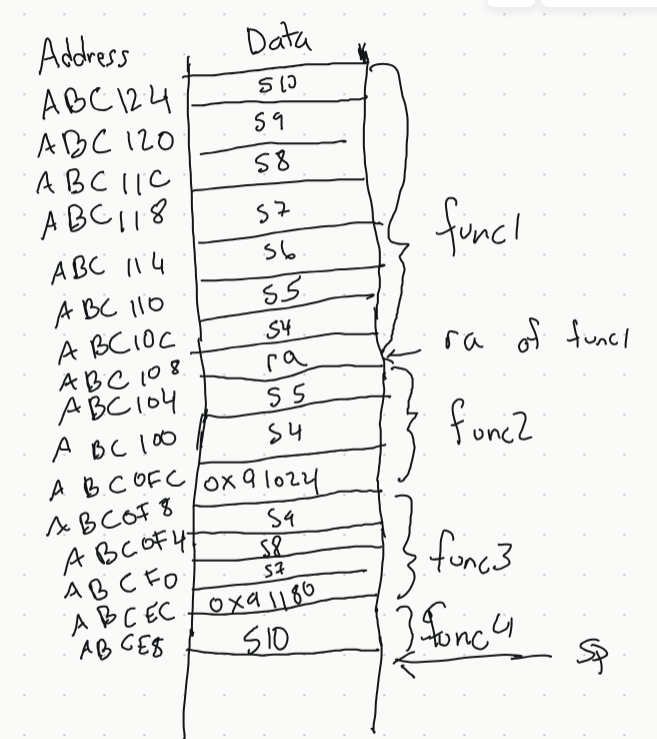
\includegraphics[width=0.5\textwidth]{exercise-6-18-stack-frame}
			\caption{Exercise 6.18: Stack frame after calling \texttt{func4}}
			\label{ex:6-18}
		\end{figure}
	\end{enumerate}
\end{sol}

\begin{ex}{6.19}
	Each number in the Fibonacci series is the sum of the two previous two
	numbers. The following table lists the first few numbers in the sequence,
	\texttt{fib(n)}.
	\begin{center}
		\begin{tabular}{c|ccccccccccc}
			\hline
			$n$ & 1 & 2 & 3 & 4 & 5 & 6 & 7 & 8 & 9 & 10 & 11\\
			\hline
			\texttt{fib(n)} & 1 & 1 & 2 & 3 & 5 & 8 & 13 & 21 & 34 & 55 & 89\\
			\hline
		\end{tabular}
	\end{center}
	\begin{enumerate}[label=(\alph*)]
		\item What is \texttt{fib(n)} for $n=0$ and $n=-1$?
		\item Write a function called \texttt{fib} in a high-level language that
		returns the Fibonacci number for any non-negative value of \texttt{n}.
		Hint: You probably will want to use a loop. Clearly comment your code.
		\item Convert the high-level function of part (b) into RISC-V assembly
		code. Add comments after every line that explain clearly what it does.
		Use a simulator to test your code on \texttt{fib(9)}. (See the preface for
		links to a RISC-V simulator).
	\end{enumerate}
\end{ex}

\begin{sol}
	\
	\begin{enumerate}[label=(\alph*)]
		\item \texttt{fib(n)} is not defined for $n=0$ or $n=-1$; it is only
		defined for non-negative integers.
		\item The following is a rudimentary implementation of \texttt{fib(n)} in C:
		\begin{lstlisting}
/* fib: Returns the n-th Fibonacci term for non-negative n; returns -1 on bad input or overflow */
long fib(long n) {
	if (n <= 0)		# Bad input
		return -1;
	long f0 = 0;
	long f1 = 1;
	for (long m = 1; m < n && f1 >= f0; m++) {
		long temp = f1;
		f1 += f0;
		f0 = temp;
	}
	if (f1 <= f0)		# Overflow
		return -1;
	return f1;
}
		\end{lstlisting}
		\item 
		\
		\begin{lstlisting}[language={}]
.globl main
main:
	addi	a0,zero,9
	jal		fib
	jr		ra
	# long fib(long n);
fib:
	bge		zero,a0,.failed	# if n <= 0 goto .failed
	addi	t0,zero,0		# f0 = 0
	addi	t1,zero,1		# f1 = 1
	addi	t2,zero,1		# m = 1
.loop:
	bge		t2,a0,.end		# if m >= n
	blt		t1,t0,.failed	# if f0 >= f1 goto .end
	addi	t3,t1,0			# temp = f1;
	add		t1,t1,t0		# t1 = t1 + t0
	addi	t0,t3,0			# t0 = temp
	addi	t2,t2,1			# m++
	j		.loop			# repeat
.end:
	bge		t0,t1,.failed	# if f0 >= f1 goto .failed
	addi	a0,t1,0			# set f1 as return value
	jr		ra				# return
.failed:
	addi	a0,zero,-1	# return -1;
	jr		ra
		\end{lstlisting}
	When run at \texttt{https://venus.kvakil.me/}, it placed \texttt{0x22} in register \texttt{a0}, which gives 34.
	\end{enumerate}
\end{sol}

\begin{ex}{6.20}
	Consider Code Example 6.28. For this exercise, assume \emph{factorial(n)}
	is called with input argument \texttt{n = 5}.
	\begin{enumerate}[label=(\alph*)]
		\item What value is in \texttt{a0} when \texttt{factorial} returns
		to the calling function?
		\item Suppose you replace the instructions at address \texttt{0x8508} and
		\texttt{0x852C} with nops. Will the program:
		\begin{enumerate}[label=(\arabic*)]
			\item Enter an infinite loop but not crash;
			\item crash (cause the stack to grow or shrink beyond the dynamic data
			segment or the PC to jump to a location outside the program);
			\item produce an incorrect value in \texttt{a0} when the program
			returns to loop (if so, what value?); or
			\item run correctly despite the deleted lines?
		\end{enumerate}
		\item Repeat part (b) with the following instruction modifications:
		\begin{enumerate}[label=(\arabic*)]
			\item Replace the instructions at addresses \texttt{0x8504} and 
			\texttt{0x8528} with nops.
			\item Replace the instruction at address \texttt{0x8518} with a nop.
			\item Replace the instruction at address \texttt{0x8530} with a nop.
		\end{enumerate}
	\end{enumerate}
\end{ex}

\begin{sol}
	\
	The code for factorial is below:
	\begin{lstlisting}[language={}]
factorial:
0x8500:	addi	sp,	sp,		-8		# make room for a0, ra
0x8504:	sw		a0	4(sp)
0x8508:	sw		ra,	0(sp)
0x850C:	addi	t0,	zero,	1		# temporary = 1
0x8510:	bgt		a0,	t0,		else	# if n>1 goto else
0x8514:	addi	a0,	zero,	1		# otherwise return 1
0x8518:	addi	sp,	sp,		8		# restore sp
0x851C:	jr		ra					# return
else:
0x8520:	addi	a0,	a0,		-1		# n = n - 1
0x8524:	jal		factorial			# recursive call
0x8528:	lw		t1,	4(sp)			# restore n into t1
0x852C:	lw		ra,	0(sp)			# restore ra
0x8530:	addi	sp,	sp,		8		# restore sp
0x8534:	mul		a0,	t1,		a0		# a0 = n * factorial(n-1)
0x8538:	jr		ra					# return
	\end{lstlisting}
	\begin{enumerate}[label=(\alph*)]
		\item \texttt{a0} will have the value $5!=120$.
		\item Instruction \texttt{0x8508} pushes the \texttt{ra} register
		onto the stack in case the function recursively calls itself. Instruction
		\texttt{0x8528} restores loads \texttt{n} from the stack onto 
		register \texttt{t1}.
		
		\
		When the function is called with \texttt{n} set to 5, it calls itself
		recursively without storing \texttt{ra} on the stack. However, the
		\texttt{jal factorial} instruction at each recursion level overwrites
		\texttt{ra}. This means that when it reaches the base case, calling itself
		with \texttt{n} set to 1, it returns to the level where \texttt{n} is 2,
		and then the instruction at address \texttt{0x852C}, namely
		\texttt{lw ra, 0(sp)}, will fail to find an address at that location.
		Since that stack address was not initialized (as a consequence of making
		\texttt{0x8058} a nop), it may have an existing value that is invalid,
		causing the program to crash because the PC will jump to a location outside
		the program.
		\item If \texttt{0x8504} and \texttt{0x8528} are replaced with nops,
		then when we get to the instruction at address \texttt{0x8534} to compute
		\texttt{n * factorial(n-1)}, register \texttt{t1} will not have
		the expect value \texttt{n}. Suppose that \texttt{t1} had value
		$x$ before \texttt{factorial(5)} was called. An incorrect value will be
		produced in \texttt{a0} when all \texttt{factorial(5)} returns, namely
		$x^4$, assuming no overflow.
		
		\
		If the instruction at \texttt{0x8518} is replaced with a nop, then the base
		case will not restore the stack pointer. When the instruction at address
		\texttt{0x852C} is executed, \texttt{factorial(2)} will return to
		address \texttt{0x8528} again as it should. However, \texttt{factorial(2)}
		will return 1 instead of 2, and similarly, \texttt{factorial(3)}
		will return 2, \texttt{factorial(4)} will return 6, and instead of ending,
		\texttt{factorial(5)} will jump again to \texttt{0x8528}, computing one
		more iteration. This time it will find \texttt{5} at \texttt{4(sp)}.
		Surprisingly, it will compute the correct return value.
		
		\
		The instruction at \texttt{0x8530} restores the stack pointer when
		a non-leaf instance of \texttt{factorial} is about to return.
		This means that \texttt{factorial(2)} will return to \texttt{factorial(3)}
		but \texttt{factorial(3)} will see the same stack values that
		\texttt{factorial(2)} saw. The code results in an infinite loop.
	\end{enumerate}
\end{sol}
\end{document}